\chapter{MATHEMATICAL DERIVATIONS}
This chapter provides the detailed mathematical framework for the fine-tuning process and the optimization algorithms used in the project.

\section{Low-Rank Adaptation (LoRA) Derivation}
In our project, we utilize LoRA to adapt Llama-2-7B. For a pre-trained weight matrix $W_0 \in \mathbb{R}^{d \times k}$, the update is constrained by a low-rank decomposition.
The forward pass for a given input $x$ is defined as:
\[
h = W_0x + \Delta Wx = W_0x + BAx
\]
Where $B \in \mathbb{R}^{d \times r}$ and $A \in \mathbb{R}^{r \times k}$, with the rank $r \ll \min(d, k)$. 
During training, $W_0$ is frozen, and only $A$ and $B$ receive gradient updates. The number of trainable parameters is reduced from $d \times k$ to $r \times (d + k)$.

\section{Cross-Entropy Loss for Code Generation}
The model is trained using the Categorical Cross-Entropy loss function to predict the next token in a code sequence. Given a sequence of tokens $y$, the loss $\mathcal{L}$ is:
\[
\mathcal{L} = -\sum_{i=1}^{V} y_i \log(\hat{y}_i)
\]
Where $V$ is the vocabulary size, $y_i$ is the ground truth (one-hot encoded), and $\hat{y}_i$ is the probability predicted by the Softmax layer:
\[
\hat{y}_i = \frac{\exp(z_i)}{\sum_{j=1}^{V} \exp(z_j)}
\]


\chapter{PROJECT BUDGET}
The project budget is primarily allocated toward high-performance compute resources required for fine-tuning the 7-billion parameter model and the development of the local inference application.

\section{Software and Cloud Services}
Since the project utilizes open-source models (Llama-2, Qwen-2.5) and open-source libraries (Transformers, PEFT, TRL), the primary cost is hardware acceleration.

\begin{table}[H]
    \centering
    \small
    \caption{Estimated Cost Breakdown}
    \begin{tabular}{p{2.7cm}p{6.5cm}p{2.5cm}}
        \toprule
        \textbf{Category} & \textbf{Item/Description} & \textbf{Estimated Cost} \\
        \midrule
        Development & Python, Ollama, PyTorch, Hugging Face API (Open Source) & Free \\
        Cloud Compute & \textbf{Google Colab Pro / RunPod}: \newline
        - NVIDIA A100 (40GB) for Fine-tuning \newline
        - NVIDIA L4 for dataset classification & \$150 - \$200 \\
        Storage & Hugging Face Hub (Model Versioning) and Drive & \$20 \\
        Miscellaneous & Documentation, LaTeX Overleaf Premium (1 Month) & \$15 \\
        \midrule
        \multicolumn{2}{l}{\textbf{Total Estimated Cost}} & \textbf{\$185 - \$235} \\
        \bottomrule
    \end{tabular}
    \label{tab:project_budget_final}
\end{table}

\chapter{PROJECT TIMELINE}
The development followed a 6-month trajectory, from data acquisition to local deployment.

\section{Gantt Chart}
The following phases were executed:
\begin{figure}[H]
    \centering
    \caption{Project Schedule (Gantt Chart)}
    \vspace{5pt} % Minimal spacing after caption
    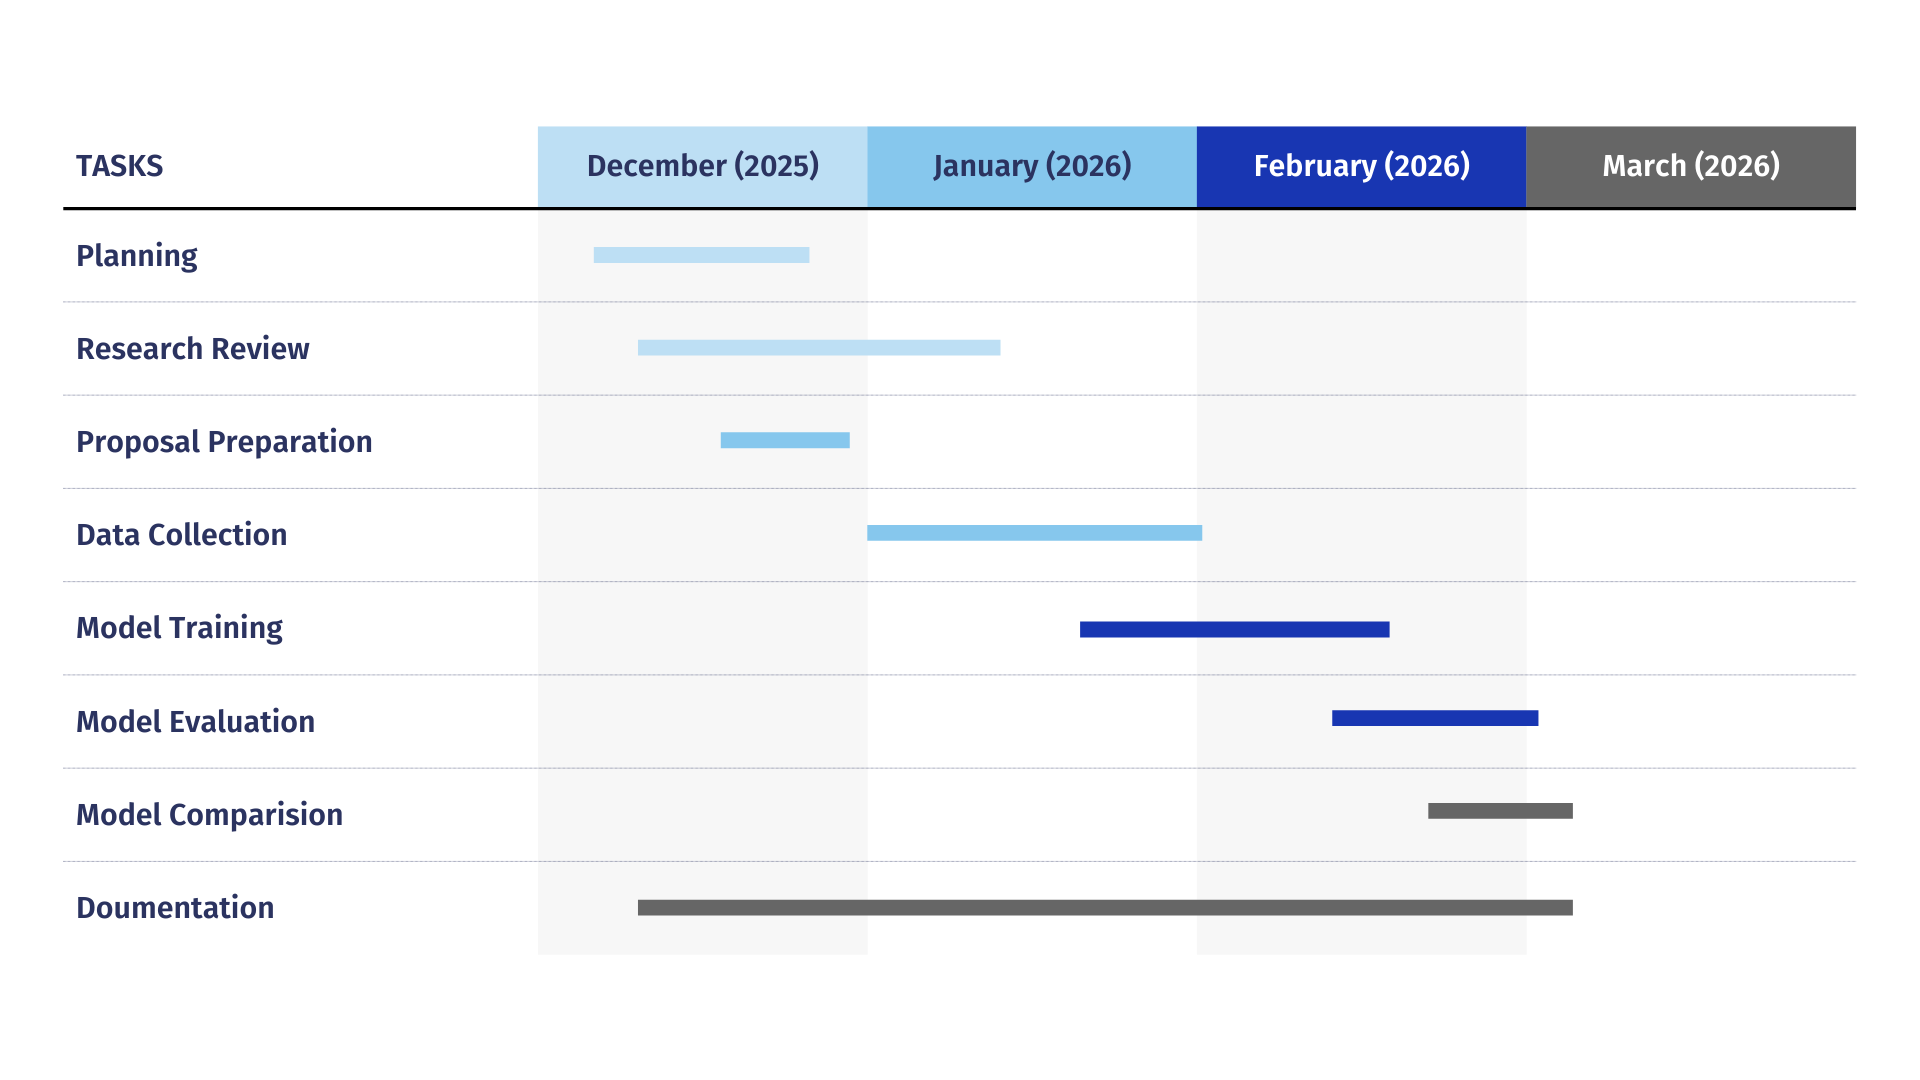
\includegraphics[width=1\textwidth]{src/images/figures/Planning.png}
    \label{fig:project_schedule}
\end{figure}



\chapter{PLAGIARISM SUMMARY}
% The student should insert the official university plagiarism report pages here.
The following pages contain the official plagiarism summary report generated by [Turnitin/Ouriginal] as provided by the university.